\documentclass[twoside]{book}

% Packages required by doxygen
\usepackage{fixltx2e}
\usepackage{calc}
\usepackage{doxygen}
\usepackage[export]{adjustbox} % also loads graphicx
\usepackage{graphicx}
\usepackage[utf8]{inputenc}
\usepackage{makeidx}
\usepackage{multicol}
\usepackage{multirow}
\PassOptionsToPackage{warn}{textcomp}
\usepackage{textcomp}
\usepackage[nointegrals]{wasysym}
\usepackage[table]{xcolor}

% Font selection
\usepackage[T1]{fontenc}
\usepackage[scaled=.90]{helvet}
\usepackage{courier}
\usepackage{amssymb}
\usepackage{sectsty}
\renewcommand{\familydefault}{\sfdefault}
\allsectionsfont{%
  \fontseries{bc}\selectfont%
  \color{darkgray}%
}
\renewcommand{\DoxyLabelFont}{%
  \fontseries{bc}\selectfont%
  \color{darkgray}%
}
\newcommand{\+}{\discretionary{\mbox{\scriptsize$\hookleftarrow$}}{}{}}

% Page & text layout
\usepackage{geometry}
\geometry{%
  a4paper,%
  top=2.5cm,%
  bottom=2.5cm,%
  left=2.5cm,%
  right=2.5cm%
}
\tolerance=750
\hfuzz=15pt
\hbadness=750
\setlength{\emergencystretch}{15pt}
\setlength{\parindent}{0cm}
\setlength{\parskip}{3ex plus 2ex minus 2ex}
\makeatletter
\renewcommand{\paragraph}{%
  \@startsection{paragraph}{4}{0ex}{-1.0ex}{1.0ex}{%
    \normalfont\normalsize\bfseries\SS@parafont%
  }%
}
\renewcommand{\subparagraph}{%
  \@startsection{subparagraph}{5}{0ex}{-1.0ex}{1.0ex}{%
    \normalfont\normalsize\bfseries\SS@subparafont%
  }%
}
\makeatother

% Headers & footers
\usepackage{fancyhdr}
\pagestyle{fancyplain}
\fancyhead[LE]{\fancyplain{}{\bfseries\thepage}}
\fancyhead[CE]{\fancyplain{}{}}
\fancyhead[RE]{\fancyplain{}{\bfseries\leftmark}}
\fancyhead[LO]{\fancyplain{}{\bfseries\rightmark}}
\fancyhead[CO]{\fancyplain{}{}}
\fancyhead[RO]{\fancyplain{}{\bfseries\thepage}}
\fancyfoot[LE]{\fancyplain{}{}}
\fancyfoot[CE]{\fancyplain{}{}}
\fancyfoot[RE]{\fancyplain{}{\bfseries\scriptsize Generated by Doxygen }}
\fancyfoot[LO]{\fancyplain{}{\bfseries\scriptsize Generated by Doxygen }}
\fancyfoot[CO]{\fancyplain{}{}}
\fancyfoot[RO]{\fancyplain{}{}}
\renewcommand{\footrulewidth}{0.4pt}
\renewcommand{\chaptermark}[1]{%
  \markboth{#1}{}%
}
\renewcommand{\sectionmark}[1]{%
  \markright{\thesection\ #1}%
}

% Indices & bibliography
\usepackage{natbib}
\usepackage[titles]{tocloft}
\setcounter{tocdepth}{3}
\setcounter{secnumdepth}{5}
\makeindex

% Hyperlinks (required, but should be loaded last)
\usepackage{ifpdf}
\ifpdf
  \usepackage[pdftex,pagebackref=true]{hyperref}
\else
  \usepackage[ps2pdf,pagebackref=true]{hyperref}
\fi
\hypersetup{%
  colorlinks=true,%
  linkcolor=blue,%
  citecolor=blue,%
  unicode%
}

% Custom commands
\newcommand{\clearemptydoublepage}{%
  \newpage{\pagestyle{empty}\cleardoublepage}%
}

\usepackage{caption}
\captionsetup{labelsep=space,justification=centering,font={bf},singlelinecheck=off,skip=4pt,position=top}

%===== C O N T E N T S =====

\begin{document}

% Titlepage & ToC
\hypersetup{pageanchor=false,
             bookmarksnumbered=true,
             pdfencoding=unicode
            }
\pagenumbering{roman}
\begin{titlepage}
\vspace*{7cm}
\begin{center}%
{\Large My Project }\\
\vspace*{1cm}
{\large Generated by Doxygen 1.8.11}\\
\end{center}
\end{titlepage}
\clearemptydoublepage
\tableofcontents
\clearemptydoublepage
\pagenumbering{arabic}
\hypersetup{pageanchor=true}

%--- Begin generated contents ---
\chapter{Class Index}
\section{Class List}
Here are the classes, structs, unions and interfaces with brief descriptions\+:\begin{DoxyCompactList}
\item\contentsline{section}{\hyperlink{classBoid}{Boid} }{\pageref{classBoid}}{}
\item\contentsline{section}{\hyperlink{classFlock}{Flock} }{\pageref{classFlock}}{}
\item\contentsline{section}{\hyperlink{classmyvector}{myvector} }{\pageref{classmyvector}}{}
\item\contentsline{section}{\hyperlink{classSimulate}{Simulate} }{\pageref{classSimulate}}{}
\end{DoxyCompactList}

\chapter{File Index}
\section{File List}
Here is a list of all documented files with brief descriptions\+:\begin{DoxyCompactList}
\item\contentsline{section}{\hyperlink{Boid_8cpp}{Boid.\+cpp} }{\pageref{Boid_8cpp}}{}
\item\contentsline{section}{\hyperlink{Boid_8h}{Boid.\+h} }{\pageref{Boid_8h}}{}
\item\contentsline{section}{\hyperlink{Flock_8cpp}{Flock.\+cpp} }{\pageref{Flock_8cpp}}{}
\item\contentsline{section}{\hyperlink{Flock_8h}{Flock.\+h} }{\pageref{Flock_8h}}{}
\item\contentsline{section}{\hyperlink{main_8cpp}{main.\+cpp} }{\pageref{main_8cpp}}{}
\end{DoxyCompactList}

\chapter{Class Documentation}
\hypertarget{classBoid}{}\section{Boid Class Reference}
\label{classBoid}\index{Boid@{Boid}}


{\ttfamily \#include $<$Boid.\+h$>$}



Collaboration diagram for Boid\+:\nopagebreak
\begin{figure}[H]
\begin{center}
\leavevmode
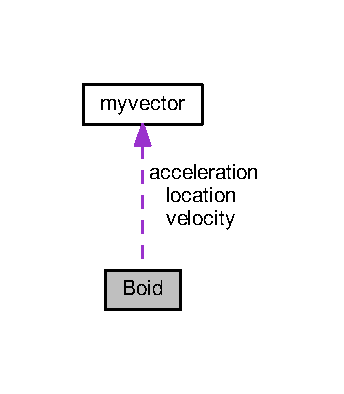
\includegraphics[width=165pt]{classBoid__coll__graph}
\end{center}
\end{figure}
\subsection*{Public Member Functions}
\begin{DoxyCompactItemize}
\item 
\hyperlink{classBoid_a5a0e15d769fc6831b6ad5c36135d7a83}{Boid} ()
\item 
\hyperlink{classBoid_a61c7081f12c16ba99dc4b3c094195bb2}{Boid} (float x, float y)
\item 
void \hyperlink{classBoid_ad73e4b8c1af1ed53cd6e5b4fd020c81e}{apply\+Force} (\hyperlink{classmyvector}{myvector} force)
\item 
\hyperlink{classmyvector}{myvector} \hyperlink{classBoid_a00eab0293372dcac7379d4deec39b430}{Separation} (vector$<$ \hyperlink{classBoid}{Boid} $>$ Boids)
\item 
\hyperlink{classmyvector}{myvector} \hyperlink{classBoid_a955a16c0223345823aadbe4493b0e982}{Alignment} (vector$<$ \hyperlink{classBoid}{Boid} $>$ Boids)
\item 
\hyperlink{classmyvector}{myvector} \hyperlink{classBoid_af8bff195217c6fd82ad390282d12f427}{Cohesion} (vector$<$ \hyperlink{classBoid}{Boid} $>$ Boids)
\item 
void \hyperlink{classBoid_ad7577660df05b58b00449c12cbc9ecdd}{run} (vector$<$ \hyperlink{classBoid}{Boid} $>$ v, int a)
\item 
void \hyperlink{classBoid_a7404d18dcb7dfc669e80c534819fa893}{update} ()
\item 
void \hyperlink{classBoid_ab8696c8548189dba88f59d917a2212fb}{flock} (vector$<$ \hyperlink{classBoid}{Boid} $>$ v)
\item 
void \hyperlink{classBoid_af1bc54215ea897a0ae4b92048073d863}{borders} (int a)
\item 
float \hyperlink{classBoid_aa5a1ed6464e44da8bef955e848635739}{angle} (\hyperlink{classmyvector}{myvector} v)
\end{DoxyCompactItemize}
\subsection*{Public Attributes}
\begin{DoxyCompactItemize}
\item 
\hyperlink{classmyvector}{myvector} \hyperlink{classBoid_a1494747f6a02c9117b581bd7f77b0c27}{location}
\item 
\hyperlink{classmyvector}{myvector} \hyperlink{classBoid_a485c85be8c3f465a2a0f07de3e0449e0}{velocity}
\item 
\hyperlink{classmyvector}{myvector} \hyperlink{classBoid_aea00ef84171ec7ae51a5d299001c673b}{acceleration}
\item 
float \hyperlink{classBoid_ac57e1058fb698a542990405ecfd1d88b}{max\+Speed}
\item 
float \hyperlink{classBoid_a2a6d579118276efaeac7ba0e4b872afd}{max\+Force}
\end{DoxyCompactItemize}


\subsection{Detailed Description}
Class for representing each boid(\+Starling). This class completely characterizes a starling. It consists of various data members like location, velocity, acceleration and many functions to maipulate these appropriately. 

\subsection{Constructor \& Destructor Documentation}
\index{Boid@{Boid}!Boid@{Boid}}
\index{Boid@{Boid}!Boid@{Boid}}
\subsubsection[{\texorpdfstring{Boid()}{Boid()}}]{\setlength{\rightskip}{0pt plus 5cm}Boid\+::\+Boid (
\begin{DoxyParamCaption}
{}
\end{DoxyParamCaption}
)\hspace{0.3cm}{\ttfamily [inline]}}\hypertarget{classBoid_a5a0e15d769fc6831b6ad5c36135d7a83}{}\label{classBoid_a5a0e15d769fc6831b6ad5c36135d7a83}
A Constructor. The default constructor(with no parameters). \index{Boid@{Boid}!Boid@{Boid}}
\index{Boid@{Boid}!Boid@{Boid}}
\subsubsection[{\texorpdfstring{Boid(float x, float y)}{Boid(float x, float y)}}]{\setlength{\rightskip}{0pt plus 5cm}Boid\+::\+Boid (
\begin{DoxyParamCaption}
\item[{float}]{x, }
\item[{float}]{y}
\end{DoxyParamCaption}
)}\hypertarget{classBoid_a61c7081f12c16ba99dc4b3c094195bb2}{}\label{classBoid_a61c7081f12c16ba99dc4b3c094195bb2}
A Constructor. The constructor initialies the a boid(\+Starling). Initializes the location, acceleration and velocity of the boid. Also defines the maxforce and maxspeed for realistic values. 

\subsection{Member Function Documentation}
\index{Boid@{Boid}!Alignment@{Alignment}}
\index{Alignment@{Alignment}!Boid@{Boid}}
\subsubsection[{\texorpdfstring{Alignment(vector$<$ Boid $>$ Boids)}{Alignment(vector< Boid > Boids)}}]{\setlength{\rightskip}{0pt plus 5cm}{\bf myvector} Boid\+::\+Alignment (
\begin{DoxyParamCaption}
\item[{vector$<$ {\bf Boid} $>$}]{boids}
\end{DoxyParamCaption}
)}\hypertarget{classBoid_a955a16c0223345823aadbe4493b0e982}{}\label{classBoid_a955a16c0223345823aadbe4493b0e982}
A Member function implementing the A\+L\+I\+G\+N\+M\+E\+NT \hyperlink{classBoid}{Boid} rule! This function instead of affecting the position of the boid, changes the velocity of the boid and add up the velocity of all the neighbouring boids, and divide it by the number of neighbours. The final value modifies the velocity instead of replacing it altogether. 
\begin{DoxyParams}{Parameters}
{\em boids} & A vector$<$\+Boid$>$ of boids. \\
\hline
\end{DoxyParams}
\begin{DoxyReturn}{Returns}
A vector which is the steer vector(Desired -\/ Velocity). 
\end{DoxyReturn}
\index{Boid@{Boid}!angle@{angle}}
\index{angle@{angle}!Boid@{Boid}}
\subsubsection[{\texorpdfstring{angle(myvector v)}{angle(myvector v)}}]{\setlength{\rightskip}{0pt plus 5cm}float Boid\+::angle (
\begin{DoxyParamCaption}
\item[{{\bf myvector}}]{v}
\end{DoxyParamCaption}
)}\hypertarget{classBoid_aa5a1ed6464e44da8bef955e848635739}{}\label{classBoid_aa5a1ed6464e44da8bef955e848635739}
A Member function which computes the angle of velocity so that image roates appropriately in the direction of motion Tan inverse x/y is returned in degrees. 
\begin{DoxyParams}{Parameters}
{\em v} & The myvector on which computation is to be done. \\
\hline
\end{DoxyParams}
\begin{DoxyReturn}{Returns}
A float representing the angle in degrees. 
\end{DoxyReturn}
\index{Boid@{Boid}!apply\+Force@{apply\+Force}}
\index{apply\+Force@{apply\+Force}!Boid@{Boid}}
\subsubsection[{\texorpdfstring{apply\+Force(myvector force)}{applyForce(myvector force)}}]{\setlength{\rightskip}{0pt plus 5cm}void Boid\+::apply\+Force (
\begin{DoxyParamCaption}
\item[{{\bf myvector}}]{force}
\end{DoxyParamCaption}
)}\hypertarget{classBoid_ad73e4b8c1af1ed53cd6e5b4fd020c81e}{}\label{classBoid_ad73e4b8c1af1ed53cd6e5b4fd020c81e}
A Member function which adds a particualr force to the boid. So this function the force vector to the current acceleration vector. 
\begin{DoxyParams}{Parameters}
{\em force} & The force vector( an object of myvector) \\
\hline
\end{DoxyParams}
\index{Boid@{Boid}!borders@{borders}}
\index{borders@{borders}!Boid@{Boid}}
\subsubsection[{\texorpdfstring{borders(int a)}{borders(int a)}}]{\setlength{\rightskip}{0pt plus 5cm}void Boid\+::borders (
\begin{DoxyParamCaption}
\item[{int}]{a}
\end{DoxyParamCaption}
)}\hypertarget{classBoid_af1bc54215ea897a0ae4b92048073d863}{}\label{classBoid_af1bc54215ea897a0ae4b92048073d863}
A Member functionis used to handle if a bird goes out of window. Depending on the input it eitheer implements wrap around or the boundary condition. 
\begin{DoxyParams}{Parameters}
{\em a} & An in which is non-\/zero when use wants wrap-\/around simulation else 0 when Boundary conditions are imposed. \\
\hline
\end{DoxyParams}
\index{Boid@{Boid}!Cohesion@{Cohesion}}
\index{Cohesion@{Cohesion}!Boid@{Boid}}
\subsubsection[{\texorpdfstring{Cohesion(vector$<$ Boid $>$ Boids)}{Cohesion(vector< Boid > Boids)}}]{\setlength{\rightskip}{0pt plus 5cm}{\bf myvector} Boid\+::\+Cohesion (
\begin{DoxyParamCaption}
\item[{vector$<$ {\bf Boid} $>$}]{boids}
\end{DoxyParamCaption}
)}\hypertarget{classBoid_af8bff195217c6fd82ad390282d12f427}{}\label{classBoid_af8bff195217c6fd82ad390282d12f427}
A Member function implementing the C\+O\+H\+E\+S\+H\+I\+ON \hyperlink{classBoid}{Boid} rule! Finds the average location of nearby boids and manipulates the steering force to move in that direction. 
\begin{DoxyParams}{Parameters}
{\em boids} & A vector$<$\+Boid$>$ of boids. \\
\hline
\end{DoxyParams}
\begin{DoxyReturn}{Returns}
A vector which is the steer vector(Desired -\/ Velocity). 
\end{DoxyReturn}
\index{Boid@{Boid}!flock@{flock}}
\index{flock@{flock}!Boid@{Boid}}
\subsubsection[{\texorpdfstring{flock(vector$<$ Boid $>$ v)}{flock(vector< Boid > v)}}]{\setlength{\rightskip}{0pt plus 5cm}void Boid\+::flock (
\begin{DoxyParamCaption}
\item[{vector$<$ {\bf Boid} $>$}]{v}
\end{DoxyParamCaption}
)}\hypertarget{classBoid_ab8696c8548189dba88f59d917a2212fb}{}\label{classBoid_ab8696c8548189dba88f59d917a2212fb}
A Member function which applies the three laws to the flock of boids. This then also assigns factors(weightage) to different laws. 
\begin{DoxyParams}{Parameters}
{\em v} & The vector of the \hyperlink{classBoid}{Boid} at the current instant. \\
\hline
\end{DoxyParams}
\begin{DoxySeeAlso}{See also}
\hyperlink{classBoid_a00eab0293372dcac7379d4deec39b430}{Separation} 

\hyperlink{classBoid_af8bff195217c6fd82ad390282d12f427}{Cohesion} 

\hyperlink{classBoid_a955a16c0223345823aadbe4493b0e982}{Alignment} 
\end{DoxySeeAlso}
\index{Boid@{Boid}!run@{run}}
\index{run@{run}!Boid@{Boid}}
\subsubsection[{\texorpdfstring{run(vector$<$ Boid $>$ v, int a)}{run(vector< Boid > v, int a)}}]{\setlength{\rightskip}{0pt plus 5cm}void Boid\+::run (
\begin{DoxyParamCaption}
\item[{vector$<$ {\bf Boid} $>$}]{v, }
\item[{int}]{a}
\end{DoxyParamCaption}
)}\hypertarget{classBoid_ad7577660df05b58b00449c12cbc9ecdd}{}\label{classBoid_ad7577660df05b58b00449c12cbc9ecdd}
A Member function which updated the parameters of the all the boids and applies the rules on them. This function updates the behaviour of the all the boids. 
\begin{DoxyParams}{Parameters}
{\em v} & The vector of the \hyperlink{classBoid}{Boid} at the current instant. \\
\hline
{\em a} & An int specifying wrap around or boundary simulation. \\
\hline
\end{DoxyParams}
\begin{DoxySeeAlso}{See also}
\hyperlink{classBoid_ab8696c8548189dba88f59d917a2212fb}{flock} 

\hyperlink{classBoid_a7404d18dcb7dfc669e80c534819fa893}{update} 

\hyperlink{classBoid_af1bc54215ea897a0ae4b92048073d863}{borders} 
\end{DoxySeeAlso}
\index{Boid@{Boid}!Separation@{Separation}}
\index{Separation@{Separation}!Boid@{Boid}}
\subsubsection[{\texorpdfstring{Separation(vector$<$ Boid $>$ Boids)}{Separation(vector< Boid > Boids)}}]{\setlength{\rightskip}{0pt plus 5cm}{\bf myvector} Boid\+::\+Separation (
\begin{DoxyParamCaption}
\item[{vector$<$ {\bf Boid} $>$}]{boids}
\end{DoxyParamCaption}
)}\hypertarget{classBoid_a00eab0293372dcac7379d4deec39b430}{}\label{classBoid_a00eab0293372dcac7379d4deec39b430}
A Member function implementing the S\+E\+P\+A\+R\+A\+T\+I\+ON \hyperlink{classBoid}{Boid} rule! This rule says that the birds have to avoid collision with its neighbours. For this we have to consider a collision radius desiredsepartion such that for a bird if there is any neighbour in this radius then the bird has to go away from that neighbour. 
\begin{DoxyParams}{Parameters}
{\em boids} & A vector$<$\+Boid$>$ of boids. \\
\hline
\end{DoxyParams}
\begin{DoxyReturn}{Returns}
A vector which is the steer vector(Desired -\/ Velocity). 
\end{DoxyReturn}
\index{Boid@{Boid}!update@{update}}
\index{update@{update}!Boid@{Boid}}
\subsubsection[{\texorpdfstring{update()}{update()}}]{\setlength{\rightskip}{0pt plus 5cm}void Boid\+::update (
\begin{DoxyParamCaption}
{}
\end{DoxyParamCaption}
)}\hypertarget{classBoid_a7404d18dcb7dfc669e80c534819fa893}{}\label{classBoid_a7404d18dcb7dfc669e80c534819fa893}
A Member function which updated the parameters of the boid in response to its environment. This modifies the location, velocity and also resets the accelration according to the values returned by the the three boid rules. 

\subsection{Member Data Documentation}
\index{Boid@{Boid}!acceleration@{acceleration}}
\index{acceleration@{acceleration}!Boid@{Boid}}
\subsubsection[{\texorpdfstring{acceleration}{acceleration}}]{\setlength{\rightskip}{0pt plus 5cm}{\bf myvector} Boid\+::acceleration}\hypertarget{classBoid_aea00ef84171ec7ae51a5d299001c673b}{}\label{classBoid_aea00ef84171ec7ae51a5d299001c673b}
A public vector representing the boid\textquotesingle{}s acceleration. \index{Boid@{Boid}!location@{location}}
\index{location@{location}!Boid@{Boid}}
\subsubsection[{\texorpdfstring{location}{location}}]{\setlength{\rightskip}{0pt plus 5cm}{\bf myvector} Boid\+::location}\hypertarget{classBoid_a1494747f6a02c9117b581bd7f77b0c27}{}\label{classBoid_a1494747f6a02c9117b581bd7f77b0c27}
A public vector representing the boid\textquotesingle{}s location. \index{Boid@{Boid}!max\+Force@{max\+Force}}
\index{max\+Force@{max\+Force}!Boid@{Boid}}
\subsubsection[{\texorpdfstring{max\+Force}{maxForce}}]{\setlength{\rightskip}{0pt plus 5cm}float Boid\+::max\+Force}\hypertarget{classBoid_a2a6d579118276efaeac7ba0e4b872afd}{}\label{classBoid_a2a6d579118276efaeac7ba0e4b872afd}
A public vector representing the maxforce the boid can experience(\+To impose realistic behaviour). \index{Boid@{Boid}!max\+Speed@{max\+Speed}}
\index{max\+Speed@{max\+Speed}!Boid@{Boid}}
\subsubsection[{\texorpdfstring{max\+Speed}{maxSpeed}}]{\setlength{\rightskip}{0pt plus 5cm}float Boid\+::max\+Speed}\hypertarget{classBoid_ac57e1058fb698a542990405ecfd1d88b}{}\label{classBoid_ac57e1058fb698a542990405ecfd1d88b}
A public vector representing the maxspeed the boid can have(\+To impose realistic behaviour). \index{Boid@{Boid}!velocity@{velocity}}
\index{velocity@{velocity}!Boid@{Boid}}
\subsubsection[{\texorpdfstring{velocity}{velocity}}]{\setlength{\rightskip}{0pt plus 5cm}{\bf myvector} Boid\+::velocity}\hypertarget{classBoid_a485c85be8c3f465a2a0f07de3e0449e0}{}\label{classBoid_a485c85be8c3f465a2a0f07de3e0449e0}
A public vector representing the boid\textquotesingle{}s velocity. 

The documentation for this class was generated from the following files\+:\begin{DoxyCompactItemize}
\item 
\hyperlink{Boid_8h}{Boid.\+h}\item 
\hyperlink{Boid_8cpp}{Boid.\+cpp}\end{DoxyCompactItemize}

\hypertarget{classFlock}{}\section{Flock Class Reference}
\label{classFlock}\index{Flock@{Flock}}


{\ttfamily \#include $<$Flock.\+h$>$}

\subsection*{Public Member Functions}
\begin{DoxyCompactItemize}
\item 
\hyperlink{classFlock_a2a0a514c368e21f718ad7358ed42f3b7}{Flock} ()
\item 
\hyperlink{classBoid}{Boid} \hyperlink{classFlock_a79925dd0c9568e57417d5d459711682d}{get\+Boid} (int i)
\item 
void \hyperlink{classFlock_ad671f2430e8b980c74d9654abe9acbc9}{add\+Boid} (\hyperlink{classBoid}{Boid} b)
\item 
int \hyperlink{classFlock_ae5801b4eed7ae1e9719f50550424e8f1}{get\+Size} ()
\item 
void \hyperlink{classFlock_a334727f018265a766832e1644d4adf87}{flocking} (int a)
\end{DoxyCompactItemize}
\subsection*{Public Attributes}
\begin{DoxyCompactItemize}
\item 
vector$<$ \hyperlink{classBoid}{Boid} $>$ \hyperlink{classFlock_a5f82ca864e51913c633c2a75fe8ba854}{flock}
\end{DoxyCompactItemize}


\subsection{Detailed Description}
Class for representing the flock(group) of starlings. This class uses the \hyperlink{classBoid}{Boid} class and is used to store the boids in the flock. 

\subsection{Constructor \& Destructor Documentation}
\index{Flock@{Flock}!Flock@{Flock}}
\index{Flock@{Flock}!Flock@{Flock}}
\subsubsection[{\texorpdfstring{Flock()}{Flock()}}]{\setlength{\rightskip}{0pt plus 5cm}Flock\+::\+Flock (
\begin{DoxyParamCaption}
{}
\end{DoxyParamCaption}
)\hspace{0.3cm}{\ttfamily [inline]}}\hypertarget{classFlock_a2a0a514c368e21f718ad7358ed42f3b7}{}\label{classFlock_a2a0a514c368e21f718ad7358ed42f3b7}
A Constructor. The default constructor(with no parameters). 

\subsection{Member Function Documentation}
\index{Flock@{Flock}!add\+Boid@{add\+Boid}}
\index{add\+Boid@{add\+Boid}!Flock@{Flock}}
\subsubsection[{\texorpdfstring{add\+Boid(\+Boid b)}{addBoid(Boid b)}}]{\setlength{\rightskip}{0pt plus 5cm}void Flock\+::add\+Boid (
\begin{DoxyParamCaption}
\item[{{\bf Boid}}]{b}
\end{DoxyParamCaption}
)}\hypertarget{classFlock_ad671f2430e8b980c74d9654abe9acbc9}{}\label{classFlock_ad671f2430e8b980c74d9654abe9acbc9}
A Member function which adds the input boid to the flock(std\+::vector$<$\+Boid$>$). 
\begin{DoxyParams}{Parameters}
{\em b} & The boid to be added. \\
\hline
\end{DoxyParams}
\index{Flock@{Flock}!flocking@{flocking}}
\index{flocking@{flocking}!Flock@{Flock}}
\subsubsection[{\texorpdfstring{flocking(int a)}{flocking(int a)}}]{\setlength{\rightskip}{0pt plus 5cm}void Flock\+::flocking (
\begin{DoxyParamCaption}
\item[{int}]{a}
\end{DoxyParamCaption}
)}\hypertarget{classFlock_a334727f018265a766832e1644d4adf87}{}\label{classFlock_a334727f018265a766832e1644d4adf87}
A Member function which updates the behaviour of every single boid w.\+r.\+t its neighbourhood. It calls the run function in \hyperlink{classBoid}{Boid} class for every \hyperlink{classBoid}{Boid} in the \hyperlink{classFlock}{Flock}. 
\begin{DoxyParams}{Parameters}
{\em a} & An int to be used by the borders function in \hyperlink{classBoid}{Boid}. \\
\hline
\end{DoxyParams}
\index{Flock@{Flock}!get\+Boid@{get\+Boid}}
\index{get\+Boid@{get\+Boid}!Flock@{Flock}}
\subsubsection[{\texorpdfstring{get\+Boid(int i)}{getBoid(int i)}}]{\setlength{\rightskip}{0pt plus 5cm}{\bf Boid} Flock\+::get\+Boid (
\begin{DoxyParamCaption}
\item[{int}]{i}
\end{DoxyParamCaption}
)}\hypertarget{classFlock_a79925dd0c9568e57417d5d459711682d}{}\label{classFlock_a79925dd0c9568e57417d5d459711682d}
A Member function which returns the boid at index i of the flock. This function takes an integer i and returns the boid at that position in the flock. A greater index means the boid is added recently(By a mouse click!) in the flock. 
\begin{DoxyParams}{Parameters}
{\em i} & An int(index). \\
\hline
\end{DoxyParams}
\begin{DoxyReturn}{Returns}
The boid at index i. 
\end{DoxyReturn}
\index{Flock@{Flock}!get\+Size@{get\+Size}}
\index{get\+Size@{get\+Size}!Flock@{Flock}}
\subsubsection[{\texorpdfstring{get\+Size()}{getSize()}}]{\setlength{\rightskip}{0pt plus 5cm}int Flock\+::get\+Size (
\begin{DoxyParamCaption}
{}
\end{DoxyParamCaption}
)}\hypertarget{classFlock_ae5801b4eed7ae1e9719f50550424e8f1}{}\label{classFlock_ae5801b4eed7ae1e9719f50550424e8f1}
A Member function which return the size of the flock. \begin{DoxyReturn}{Returns}
An int representing the number of Boids in the flock at that instant. 
\end{DoxyReturn}


\subsection{Member Data Documentation}
\index{Flock@{Flock}!flock@{flock}}
\index{flock@{flock}!Flock@{Flock}}
\subsubsection[{\texorpdfstring{flock}{flock}}]{\setlength{\rightskip}{0pt plus 5cm}vector$<${\bf Boid}$>$ Flock\+::flock}\hypertarget{classFlock_a5f82ca864e51913c633c2a75fe8ba854}{}\label{classFlock_a5f82ca864e51913c633c2a75fe8ba854}
A public std\+::vector of Boids representing the floack as a whole. 

The documentation for this class was generated from the following files\+:\begin{DoxyCompactItemize}
\item 
\hyperlink{Flock_8h}{Flock.\+h}\item 
\hyperlink{Flock_8cpp}{Flock.\+cpp}\end{DoxyCompactItemize}

\hypertarget{classmyvector}{}\section{myvector Class Reference}
\label{classmyvector}\index{myvector@{myvector}}


{\ttfamily \#include $<$Boid.\+h$>$}

\subsection*{Public Member Functions}
\begin{DoxyCompactItemize}
\item 
\hyperlink{classmyvector_a14f6044bcf6e97fbe98dd5b59a91de9b}{myvector} ()
\item 
\hyperlink{classmyvector_aae4378de3a05547573e5c557547d29c6}{myvector} (float a, float b)
\item 
void \hyperlink{classmyvector_a53d8fcdcc0eaf2bef92e3a75effbb29d}{set} (float \hyperlink{classmyvector_a1e3915c15a349ccf949bb1751a5601c7}{x}, float \hyperlink{classmyvector_a44a88317051b0eacb7d9a1fb341879ae}{y})
\item 
void \hyperlink{classmyvector_a9de9660a79b1ab91b46e19764e45c762}{add\+Vector} (\hyperlink{classmyvector}{myvector} v)
\item 
void \hyperlink{classmyvector_a0d75094dd9d203f3631804c25081e6e1}{add\+Scalar} (float \hyperlink{classmyvector_a1e3915c15a349ccf949bb1751a5601c7}{x})
\item 
void \hyperlink{classmyvector_aa95fab10c88bb820a1df1a81b8a99e5a}{sub\+Vector} (\hyperlink{classmyvector}{myvector} v)
\item 
void \hyperlink{classmyvector_aae72e5012c3f1174c2088726c007b72d}{sub\+Scalar} (float \hyperlink{classmyvector_a1e3915c15a349ccf949bb1751a5601c7}{x})
\item 
void \hyperlink{classmyvector_a195cbe72f741ec0157e41682ef46955d}{mul\+Vector} (\hyperlink{classmyvector}{myvector} v)
\item 
void \hyperlink{classmyvector_a1df8c126386ada675bedcfc0d669dd9b}{mul\+Scalar} (float \hyperlink{classmyvector_a1e3915c15a349ccf949bb1751a5601c7}{x})
\item 
void \hyperlink{classmyvector_a94f0319a79e86f455620ebd972de5a51}{div\+Vector} (\hyperlink{classmyvector}{myvector} v)
\item 
void \hyperlink{classmyvector_a6f13869f698e6d04eec62eda846f1c89}{div\+Scalar} (float \hyperlink{classmyvector_a1e3915c15a349ccf949bb1751a5601c7}{x})
\item 
void \hyperlink{classmyvector_a7513dd63482f8da0391482a42ec94716}{limit} (double max)
\item 
float \hyperlink{classmyvector_a3b88ac1b07500053fcced210f919e1d2}{distance\+Two\+Vectors} (\hyperlink{classmyvector}{myvector} v)
\item 
float \hyperlink{classmyvector_aeb8789b346cb5622637bc4892ecf81f3}{dot\+Product} (\hyperlink{classmyvector}{myvector} v)
\item 
float \hyperlink{classmyvector_a262a2cb9fee43e76d047518236b24ac4}{magnitude} ()
\item 
void \hyperlink{classmyvector_a7dd9ce447a27dccec70dda20b4d6c862}{set\+Magnitude} (float \hyperlink{classmyvector_a1e3915c15a349ccf949bb1751a5601c7}{x})
\item 
float \hyperlink{classmyvector_a68e76f412562234f077583902873d14a}{angle} (\hyperlink{classmyvector}{myvector} v)
\item 
void \hyperlink{classmyvector_ac0ca9829a310802c12d3bfc246dec920}{normalize} ()
\item 
\hyperlink{classmyvector}{myvector} \hyperlink{classmyvector_a5d48deffc52b7710383eccf82581e72e}{copy} (\hyperlink{classmyvector}{myvector} v)
\end{DoxyCompactItemize}
\subsection*{Public Attributes}
\begin{DoxyCompactItemize}
\item 
float \hyperlink{classmyvector_a1e3915c15a349ccf949bb1751a5601c7}{x}
\item 
float \hyperlink{classmyvector_a44a88317051b0eacb7d9a1fb341879ae}{y}
\end{DoxyCompactItemize}


\subsection{Detailed Description}
Class for representing Euclidian vectors. The vectors have both magnitude and direction. These are used to denote the location, velocity and acceleration of each starling. 

\subsection{Constructor \& Destructor Documentation}
\index{myvector@{myvector}!myvector@{myvector}}
\index{myvector@{myvector}!myvector@{myvector}}
\subsubsection[{\texorpdfstring{myvector()}{myvector()}}]{\setlength{\rightskip}{0pt plus 5cm}myvector\+::myvector (
\begin{DoxyParamCaption}
{}
\end{DoxyParamCaption}
)\hspace{0.3cm}{\ttfamily [inline]}}\hypertarget{classmyvector_a14f6044bcf6e97fbe98dd5b59a91de9b}{}\label{classmyvector_a14f6044bcf6e97fbe98dd5b59a91de9b}
A Constructor. The default constructor(with no parameters). \index{myvector@{myvector}!myvector@{myvector}}
\index{myvector@{myvector}!myvector@{myvector}}
\subsubsection[{\texorpdfstring{myvector(float a, float b)}{myvector(float a, float b)}}]{\setlength{\rightskip}{0pt plus 5cm}myvector\+::myvector (
\begin{DoxyParamCaption}
\item[{float}]{a, }
\item[{float}]{b}
\end{DoxyParamCaption}
)\hspace{0.3cm}{\ttfamily [inline]}}\hypertarget{classmyvector_aae4378de3a05547573e5c557547d29c6}{}\label{classmyvector_aae4378de3a05547573e5c557547d29c6}
A Constructor. The constructor initialies the vector. 
\begin{DoxyParams}{Parameters}
{\em a} & the x-\/projection. \\
\hline
{\em b} & the y-\/projection. \\
\hline
\end{DoxyParams}


\subsection{Member Function Documentation}
\index{myvector@{myvector}!add\+Scalar@{add\+Scalar}}
\index{add\+Scalar@{add\+Scalar}!myvector@{myvector}}
\subsubsection[{\texorpdfstring{add\+Scalar(float x)}{addScalar(float x)}}]{\setlength{\rightskip}{0pt plus 5cm}void myvector\+::add\+Scalar (
\begin{DoxyParamCaption}
\item[{float}]{a}
\end{DoxyParamCaption}
)}\hypertarget{classmyvector_a0d75094dd9d203f3631804c25081e6e1}{}\label{classmyvector_a0d75094dd9d203f3631804c25081e6e1}
A Member function which adds a scalar( type float) from the current object. Individually increments different components of the myvetor object by the input scalar. 
\begin{DoxyParams}{Parameters}
{\em a} & A float to be added. \\
\hline
\end{DoxyParams}
\index{myvector@{myvector}!add\+Vector@{add\+Vector}}
\index{add\+Vector@{add\+Vector}!myvector@{myvector}}
\subsubsection[{\texorpdfstring{add\+Vector(myvector v)}{addVector(myvector v)}}]{\setlength{\rightskip}{0pt plus 5cm}void myvector\+::add\+Vector (
\begin{DoxyParamCaption}
\item[{{\bf myvector}}]{v}
\end{DoxyParamCaption}
)}\hypertarget{classmyvector_a9de9660a79b1ab91b46e19764e45c762}{}\label{classmyvector_a9de9660a79b1ab91b46e19764e45c762}
A Member function which adds a myvector object to the current object. Individually adds different components of the two vectors. 
\begin{DoxyParams}{Parameters}
{\em v} & A vector(object) of the myvector class. \\
\hline
\end{DoxyParams}
\index{myvector@{myvector}!angle@{angle}}
\index{angle@{angle}!myvector@{myvector}}
\subsubsection[{\texorpdfstring{angle(myvector v)}{angle(myvector v)}}]{\setlength{\rightskip}{0pt plus 5cm}float myvector\+::angle (
\begin{DoxyParamCaption}
\item[{{\bf myvector}}]{v}
\end{DoxyParamCaption}
)}\hypertarget{classmyvector_a68e76f412562234f077583902873d14a}{}\label{classmyvector_a68e76f412562234f077583902873d14a}
A Member function which computes the angle(in radians) between two vectors. 
\begin{DoxyParams}{Parameters}
{\em v} & A vector whose angle with the current vector is to be calculated. \\
\hline
\end{DoxyParams}
\begin{DoxyReturn}{Returns}
A float representing th angle between the two vectors. 
\end{DoxyReturn}
\index{myvector@{myvector}!copy@{copy}}
\index{copy@{copy}!myvector@{myvector}}
\subsubsection[{\texorpdfstring{copy(myvector v)}{copy(myvector v)}}]{\setlength{\rightskip}{0pt plus 5cm}{\bf myvector} myvector\+::copy (
\begin{DoxyParamCaption}
\item[{{\bf myvector}}]{v}
\end{DoxyParamCaption}
)}\hypertarget{classmyvector_a5d48deffc52b7710383eccf82581e72e}{}\label{classmyvector_a5d48deffc52b7710383eccf82581e72e}
A Member function which creates a copy of the input vector. \begin{DoxyReturn}{Returns}
The copy of the input vector. 
\end{DoxyReturn}
\index{myvector@{myvector}!distance\+Two\+Vectors@{distance\+Two\+Vectors}}
\index{distance\+Two\+Vectors@{distance\+Two\+Vectors}!myvector@{myvector}}
\subsubsection[{\texorpdfstring{distance\+Two\+Vectors(myvector v)}{distanceTwoVectors(myvector v)}}]{\setlength{\rightskip}{0pt plus 5cm}float myvector\+::distance\+Two\+Vectors (
\begin{DoxyParamCaption}
\item[{{\bf myvector}}]{v}
\end{DoxyParamCaption}
)}\hypertarget{classmyvector_a3b88ac1b07500053fcced210f919e1d2}{}\label{classmyvector_a3b88ac1b07500053fcced210f919e1d2}
A Member function which computes the distance between two myvectors. Calculates the distance between the input myvector and the current myvector. 
\begin{DoxyParams}{Parameters}
{\em max} & An object of myvector class. \\
\hline
\end{DoxyParams}
\begin{DoxyReturn}{Returns}
dist\+:The required distance of type float. 
\end{DoxyReturn}
\index{myvector@{myvector}!div\+Scalar@{div\+Scalar}}
\index{div\+Scalar@{div\+Scalar}!myvector@{myvector}}
\subsubsection[{\texorpdfstring{div\+Scalar(float x)}{divScalar(float x)}}]{\setlength{\rightskip}{0pt plus 5cm}void myvector\+::div\+Scalar (
\begin{DoxyParamCaption}
\item[{float}]{a}
\end{DoxyParamCaption}
)}\hypertarget{classmyvector_a6f13869f698e6d04eec62eda846f1c89}{}\label{classmyvector_a6f13869f698e6d04eec62eda846f1c89}
A Member function which divides a scalar( type float) to the current object. Individually divides different components of the myvetor object by the input scalar. 
\begin{DoxyParams}{Parameters}
{\em a} & A float to be divided by. \\
\hline
\end{DoxyParams}
\index{myvector@{myvector}!div\+Vector@{div\+Vector}}
\index{div\+Vector@{div\+Vector}!myvector@{myvector}}
\subsubsection[{\texorpdfstring{div\+Vector(myvector v)}{divVector(myvector v)}}]{\setlength{\rightskip}{0pt plus 5cm}void myvector\+::div\+Vector (
\begin{DoxyParamCaption}
\item[{{\bf myvector}}]{v}
\end{DoxyParamCaption}
)}\hypertarget{classmyvector_a94f0319a79e86f455620ebd972de5a51}{}\label{classmyvector_a94f0319a79e86f455620ebd972de5a51}
A Member function which divides a myvector object to the current object. Individually divides different components of the two vectors. 
\begin{DoxyParams}{Parameters}
{\em v} & A vector(object) of the myvector class. This function may be used when we want to scale differnt components by diff values in a go. \\
\hline
\end{DoxyParams}
\index{myvector@{myvector}!dot\+Product@{dot\+Product}}
\index{dot\+Product@{dot\+Product}!myvector@{myvector}}
\subsubsection[{\texorpdfstring{dot\+Product(myvector v)}{dotProduct(myvector v)}}]{\setlength{\rightskip}{0pt plus 5cm}float myvector\+::dot\+Product (
\begin{DoxyParamCaption}
\item[{{\bf myvector}}]{v}
\end{DoxyParamCaption}
)}\hypertarget{classmyvector_aeb8789b346cb5622637bc4892ecf81f3}{}\label{classmyvector_aeb8789b346cb5622637bc4892ecf81f3}
A Member function which calculates dot product of two vectors. Calculates dot product of the object vector and the arguement vector and returns a float value. 
\begin{DoxyParams}{Parameters}
{\em v} & A vector. \\
\hline
\end{DoxyParams}
\begin{DoxyReturn}{Returns}
The dot product(float value). 
\end{DoxyReturn}
\index{myvector@{myvector}!limit@{limit}}
\index{limit@{limit}!myvector@{myvector}}
\subsubsection[{\texorpdfstring{limit(double max)}{limit(double max)}}]{\setlength{\rightskip}{0pt plus 5cm}void myvector\+::limit (
\begin{DoxyParamCaption}
\item[{double}]{max}
\end{DoxyParamCaption}
)}\hypertarget{classmyvector_a7513dd63482f8da0391482a42ec94716}{}\label{classmyvector_a7513dd63482f8da0391482a42ec94716}
A Member function which limits the magnitude of a myvector object by a constant value. Checks if magnitude of myvector is greter than the input value. IF yes, the divides each component by that value else no chang 
\begin{DoxyParams}{Parameters}
{\em max} & A double which is used limit the myvector. \\
\hline
\end{DoxyParams}
\index{myvector@{myvector}!magnitude@{magnitude}}
\index{magnitude@{magnitude}!myvector@{myvector}}
\subsubsection[{\texorpdfstring{magnitude()}{magnitude()}}]{\setlength{\rightskip}{0pt plus 5cm}float myvector\+::magnitude (
\begin{DoxyParamCaption}
{}
\end{DoxyParamCaption}
)}\hypertarget{classmyvector_a262a2cb9fee43e76d047518236b24ac4}{}\label{classmyvector_a262a2cb9fee43e76d047518236b24ac4}
A Member function which computes the magnitude of the myvector object. \begin{DoxyReturn}{Returns}
A float representing the magnitude. 
\end{DoxyReturn}
\index{myvector@{myvector}!mul\+Scalar@{mul\+Scalar}}
\index{mul\+Scalar@{mul\+Scalar}!myvector@{myvector}}
\subsubsection[{\texorpdfstring{mul\+Scalar(float x)}{mulScalar(float x)}}]{\setlength{\rightskip}{0pt plus 5cm}void myvector\+::mul\+Scalar (
\begin{DoxyParamCaption}
\item[{float}]{a}
\end{DoxyParamCaption}
)}\hypertarget{classmyvector_a1df8c126386ada675bedcfc0d669dd9b}{}\label{classmyvector_a1df8c126386ada675bedcfc0d669dd9b}
A Member function which multiplies a scalar( type float) to the current object. Individually multiplies different components of the myvetor object by the input scalar. 
\begin{DoxyParams}{Parameters}
{\em a} & A float to be multiplied. \\
\hline
\end{DoxyParams}
\index{myvector@{myvector}!mul\+Vector@{mul\+Vector}}
\index{mul\+Vector@{mul\+Vector}!myvector@{myvector}}
\subsubsection[{\texorpdfstring{mul\+Vector(myvector v)}{mulVector(myvector v)}}]{\setlength{\rightskip}{0pt plus 5cm}void myvector\+::mul\+Vector (
\begin{DoxyParamCaption}
\item[{{\bf myvector}}]{v}
\end{DoxyParamCaption}
)}\hypertarget{classmyvector_a195cbe72f741ec0157e41682ef46955d}{}\label{classmyvector_a195cbe72f741ec0157e41682ef46955d}
A Member function which multiplies a myvector object to the current object. Individually multiplies different components of the two vectors. 
\begin{DoxyParams}{Parameters}
{\em v} & A vector(object) of the myvector class. This function may be used when we want to scale differnt components by diff values in a go. \\
\hline
\end{DoxyParams}
\index{myvector@{myvector}!normalize@{normalize}}
\index{normalize@{normalize}!myvector@{myvector}}
\subsubsection[{\texorpdfstring{normalize()}{normalize()}}]{\setlength{\rightskip}{0pt plus 5cm}void myvector\+::normalize (
\begin{DoxyParamCaption}
{}
\end{DoxyParamCaption}
)}\hypertarget{classmyvector_ac0ca9829a310802c12d3bfc246dec920}{}\label{classmyvector_ac0ca9829a310802c12d3bfc246dec920}
A Member function which normalizes the current vector. It modifies the vector to make it a unit magnitude vector. \index{myvector@{myvector}!set@{set}}
\index{set@{set}!myvector@{myvector}}
\subsubsection[{\texorpdfstring{set(float x, float y)}{set(float x, float y)}}]{\setlength{\rightskip}{0pt plus 5cm}void myvector\+::set (
\begin{DoxyParamCaption}
\item[{float}]{a, }
\item[{float}]{b}
\end{DoxyParamCaption}
)}\hypertarget{classmyvector_a53d8fcdcc0eaf2bef92e3a75effbb29d}{}\label{classmyvector_a53d8fcdcc0eaf2bef92e3a75effbb29d}
A Member function which sets the fields of an object of class myvector. 
\begin{DoxyParams}{Parameters}
{\em a} & A float representing the x component. \\
\hline
{\em b} & A float representing the y component. \\
\hline
\end{DoxyParams}
\index{myvector@{myvector}!set\+Magnitude@{set\+Magnitude}}
\index{set\+Magnitude@{set\+Magnitude}!myvector@{myvector}}
\subsubsection[{\texorpdfstring{set\+Magnitude(float x)}{setMagnitude(float x)}}]{\setlength{\rightskip}{0pt plus 5cm}void myvector\+::set\+Magnitude (
\begin{DoxyParamCaption}
\item[{float}]{x}
\end{DoxyParamCaption}
)}\hypertarget{classmyvector_a7dd9ce447a27dccec70dda20b4d6c862}{}\label{classmyvector_a7dd9ce447a27dccec70dda20b4d6c862}
A Member function which modifies the vector to have a particualr magnitude. So this function enlarges or diminishes the vector appropriately by a given a constant. 
\begin{DoxyParams}{Parameters}
{\em x} & A float to be set as the magnitude. \\
\hline
\end{DoxyParams}
\begin{DoxySeeAlso}{See also}
\hyperlink{classmyvector_ac0ca9829a310802c12d3bfc246dec920}{normalize} 

mulscalar 
\end{DoxySeeAlso}
\index{myvector@{myvector}!sub\+Scalar@{sub\+Scalar}}
\index{sub\+Scalar@{sub\+Scalar}!myvector@{myvector}}
\subsubsection[{\texorpdfstring{sub\+Scalar(float x)}{subScalar(float x)}}]{\setlength{\rightskip}{0pt plus 5cm}void myvector\+::sub\+Scalar (
\begin{DoxyParamCaption}
\item[{float}]{a}
\end{DoxyParamCaption}
)}\hypertarget{classmyvector_aae72e5012c3f1174c2088726c007b72d}{}\label{classmyvector_aae72e5012c3f1174c2088726c007b72d}
A Member function which subtracts a scalar( type float) from the current object. Individually decrements different components of the myvetor object by the input scalar. 
\begin{DoxyParams}{Parameters}
{\em a} & A float to be subtracted. \\
\hline
\end{DoxyParams}
\index{myvector@{myvector}!sub\+Vector@{sub\+Vector}}
\index{sub\+Vector@{sub\+Vector}!myvector@{myvector}}
\subsubsection[{\texorpdfstring{sub\+Vector(myvector v)}{subVector(myvector v)}}]{\setlength{\rightskip}{0pt plus 5cm}void myvector\+::sub\+Vector (
\begin{DoxyParamCaption}
\item[{{\bf myvector}}]{v}
\end{DoxyParamCaption}
)}\hypertarget{classmyvector_aa95fab10c88bb820a1df1a81b8a99e5a}{}\label{classmyvector_aa95fab10c88bb820a1df1a81b8a99e5a}
A Member function which subtracts a myvector object to the current object. Individually subtracts different components of the two vectors. 
\begin{DoxyParams}{Parameters}
{\em v} & A vector(object) of the myvector class. \\
\hline
\end{DoxyParams}


\subsection{Member Data Documentation}
\index{myvector@{myvector}!x@{x}}
\index{x@{x}!myvector@{myvector}}
\subsubsection[{\texorpdfstring{x}{x}}]{\setlength{\rightskip}{0pt plus 5cm}float myvector\+::x}\hypertarget{classmyvector_a1e3915c15a349ccf949bb1751a5601c7}{}\label{classmyvector_a1e3915c15a349ccf949bb1751a5601c7}
A public float member representing x-\/projection. \index{myvector@{myvector}!y@{y}}
\index{y@{y}!myvector@{myvector}}
\subsubsection[{\texorpdfstring{y}{y}}]{\setlength{\rightskip}{0pt plus 5cm}float myvector\+::y}\hypertarget{classmyvector_a44a88317051b0eacb7d9a1fb341879ae}{}\label{classmyvector_a44a88317051b0eacb7d9a1fb341879ae}
A public float member representing y-\/projection. 

The documentation for this class was generated from the following files\+:\begin{DoxyCompactItemize}
\item 
\hyperlink{Boid_8h}{Boid.\+h}\item 
\hyperlink{Boid_8cpp}{Boid.\+cpp}\end{DoxyCompactItemize}

\hypertarget{classSimulate}{}\section{Simulate Class Reference}
\label{classSimulate}\index{Simulate@{Simulate}}
\subsection*{Public Member Functions}
\begin{DoxyCompactItemize}
\item 
\hyperlink{classSimulate_a815c999390d9cd16e49245d4957ca946}{Simulate} ()
\item 
void \hyperlink{classSimulate_a496aa26515bbae1e48240b2e4db4eeb8}{Run} (int a)
\end{DoxyCompactItemize}
\subsection*{Public Attributes}
\begin{DoxyCompactItemize}
\item 
int \hyperlink{classSimulate_a40bb55ff98362e746ac03f2369ddac08}{Num\+\_\+boids}
\end{DoxyCompactItemize}


\subsection{Detailed Description}
Class for doing the simulation and rendering using S\+F\+ML This class handles all the input(eg. mouse clicks.). Handles all the program\textquotesingle{}s interaction with S\+F\+ML. This class contatins some private function requred for rendering and handling input too. 

\subsection{Constructor \& Destructor Documentation}
\index{Simulate@{Simulate}!Simulate@{Simulate}}
\index{Simulate@{Simulate}!Simulate@{Simulate}}
\subsubsection[{\texorpdfstring{Simulate()}{Simulate()}}]{\setlength{\rightskip}{0pt plus 5cm}Simulate\+::\+Simulate (
\begin{DoxyParamCaption}
{}
\end{DoxyParamCaption}
)\hspace{0.3cm}{\ttfamily [inline]}}\hypertarget{classSimulate_a815c999390d9cd16e49245d4957ca946}{}\label{classSimulate_a815c999390d9cd16e49245d4957ca946}
A Constructor. The constructor constructs the window and sets up the required properties of simulation. 

\subsection{Member Function Documentation}
\index{Simulate@{Simulate}!Run@{Run}}
\index{Run@{Run}!Simulate@{Simulate}}
\subsubsection[{\texorpdfstring{Run(int a)}{Run(int a)}}]{\setlength{\rightskip}{0pt plus 5cm}void Simulate\+::\+Run (
\begin{DoxyParamCaption}
\item[{int}]{a}
\end{DoxyParamCaption}
)\hspace{0.3cm}{\ttfamily [inline]}}\hypertarget{classSimulate_a496aa26515bbae1e48240b2e4db4eeb8}{}\label{classSimulate_a496aa26515bbae1e48240b2e4db4eeb8}
A Member function which runs the simulation of starlings. This simulates and displays the boids that we create and handles the reqired input. 
\begin{DoxyParams}{Parameters}
{\em a} & An int which is passed to the \hyperlink{classBoid}{Boid} class to do simulation either in a wrap around manner(when a is non-\/zero) or confined to bounderies(when a = 0). \\
\hline
\end{DoxyParams}
\begin{DoxySeeAlso}{See also}
borders 

\hyperlink{classBoid}{Boid} 
\end{DoxySeeAlso}


\subsection{Member Data Documentation}
\index{Simulate@{Simulate}!Num\+\_\+boids@{Num\+\_\+boids}}
\index{Num\+\_\+boids@{Num\+\_\+boids}!Simulate@{Simulate}}
\subsubsection[{\texorpdfstring{Num\+\_\+boids}{Num_boids}}]{\setlength{\rightskip}{0pt plus 5cm}int Simulate\+::\+Num\+\_\+boids}\hypertarget{classSimulate_a40bb55ff98362e746ac03f2369ddac08}{}\label{classSimulate_a40bb55ff98362e746ac03f2369ddac08}
A public int denoting number of starlings at any instant. 

The documentation for this class was generated from the following file\+:\begin{DoxyCompactItemize}
\item 
\hyperlink{main_8cpp}{main.\+cpp}\end{DoxyCompactItemize}

\chapter{File Documentation}
\hypertarget{Boid_8cpp}{}\section{Boid.\+cpp File Reference}
\label{Boid_8cpp}\index{Boid.\+cpp@{Boid.\+cpp}}
{\ttfamily \#include $<$iostream$>$}\\*
{\ttfamily \#include $<$vector$>$}\\*
{\ttfamily \#include $<$string$>$}\\*
{\ttfamily \#include $<$math.\+h$>$}\\*
{\ttfamily \#include \char`\"{}S\+F\+M\+L/\+Graphics.\+hpp\char`\"{}}\\*
{\ttfamily \#include \char`\"{}Boid.\+h\char`\"{}}\\*
Include dependency graph for Boid.\+cpp\+:\nopagebreak
\begin{figure}[H]
\begin{center}
\leavevmode
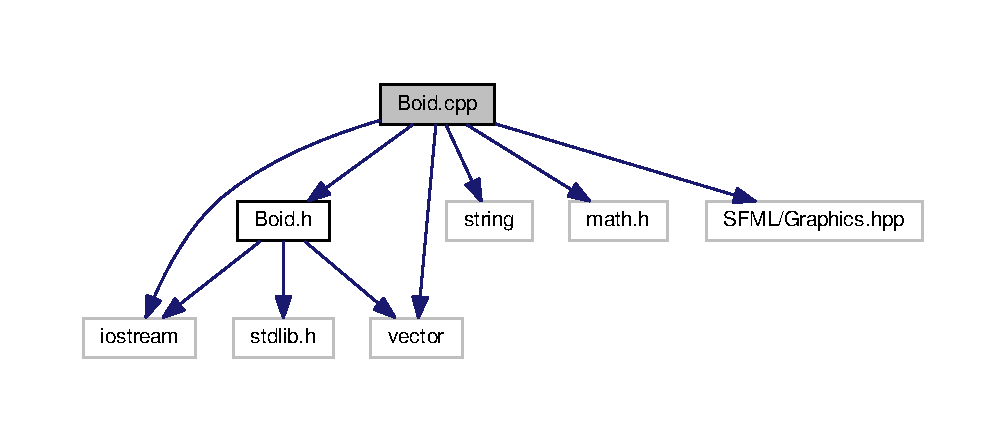
\includegraphics[width=350pt]{Boid_8cpp__incl}
\end{center}
\end{figure}
\subsection*{Macros}
\begin{DoxyCompactItemize}
\item 
\#define {\bfseries w\+\_\+height}~window\+\_\+height\hypertarget{Boid_8cpp_a303f3b558527003501377f4c2dff288e}{}\label{Boid_8cpp_a303f3b558527003501377f4c2dff288e}

\item 
\#define {\bfseries w\+\_\+width}~window\+\_\+width\hypertarget{Boid_8cpp_afa698183adde3126aa90e31286b0aef6}{}\label{Boid_8cpp_afa698183adde3126aa90e31286b0aef6}

\item 
\#define {\bfseries PI}~3.\+141592635\hypertarget{Boid_8cpp_a598a3330b3c21701223ee0ca14316eca}{}\label{Boid_8cpp_a598a3330b3c21701223ee0ca14316eca}

\end{DoxyCompactItemize}
\subsection*{Variables}
\begin{DoxyCompactItemize}
\item 
sf\+::\+Video\+Mode {\bfseries desktop\+Temp} = sf\+::\+Video\+Mode\+::get\+Desktop\+Mode()\hypertarget{Boid_8cpp_a77534fd11654e7b4832f7bace37dadf9}{}\label{Boid_8cpp_a77534fd11654e7b4832f7bace37dadf9}

\item 
const int {\bfseries window\+\_\+height} = desktop\+Temp.\+height\hypertarget{Boid_8cpp_a7be74e799254792ccf1dddce8c4cd0cb}{}\label{Boid_8cpp_a7be74e799254792ccf1dddce8c4cd0cb}

\item 
const int {\bfseries window\+\_\+width} = desktop\+Temp.\+width\hypertarget{Boid_8cpp_a39a2fe953af0d179b5a76a26458ce57e}{}\label{Boid_8cpp_a39a2fe953af0d179b5a76a26458ce57e}

\end{DoxyCompactItemize}

\hypertarget{Boid_8h}{}\section{Boid.\+h File Reference}
\label{Boid_8h}\index{Boid.\+h@{Boid.\+h}}
{\ttfamily \#include $<$vector$>$}\\*
{\ttfamily \#include $<$stdlib.\+h$>$}\\*
{\ttfamily \#include $<$iostream$>$}\\*
Include dependency graph for Boid.\+h\+:\nopagebreak
\begin{figure}[H]
\begin{center}
\leavevmode
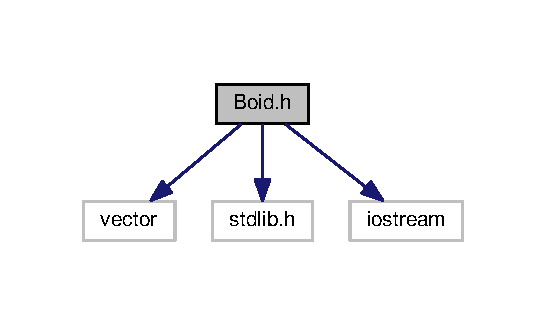
\includegraphics[width=262pt]{Boid_8h__incl}
\end{center}
\end{figure}
This graph shows which files directly or indirectly include this file\+:\nopagebreak
\begin{figure}[H]
\begin{center}
\leavevmode
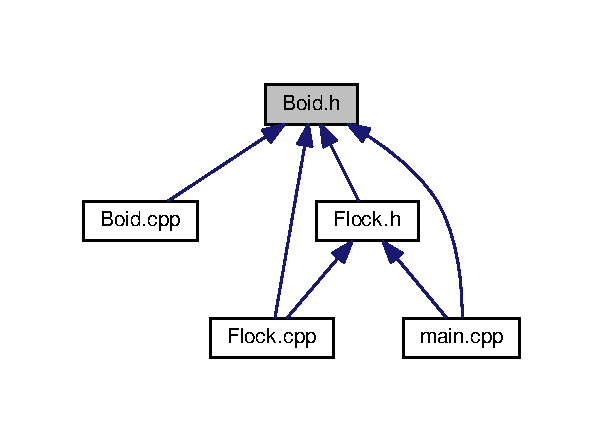
\includegraphics[width=290pt]{Boid_8h__dep__incl}
\end{center}
\end{figure}
\subsection*{Classes}
\begin{DoxyCompactItemize}
\item 
class \hyperlink{classmyvector}{myvector}
\item 
class \hyperlink{classBoid}{Boid}
\end{DoxyCompactItemize}

\hypertarget{Flock_8cpp}{}\section{Flock.\+cpp File Reference}
\label{Flock_8cpp}\index{Flock.\+cpp@{Flock.\+cpp}}
{\ttfamily \#include \char`\"{}Boid.\+h\char`\"{}}\\*
{\ttfamily \#include \char`\"{}Flock.\+h\char`\"{}}\\*
Include dependency graph for Flock.\+cpp\+:\nopagebreak
\begin{figure}[H]
\begin{center}
\leavevmode
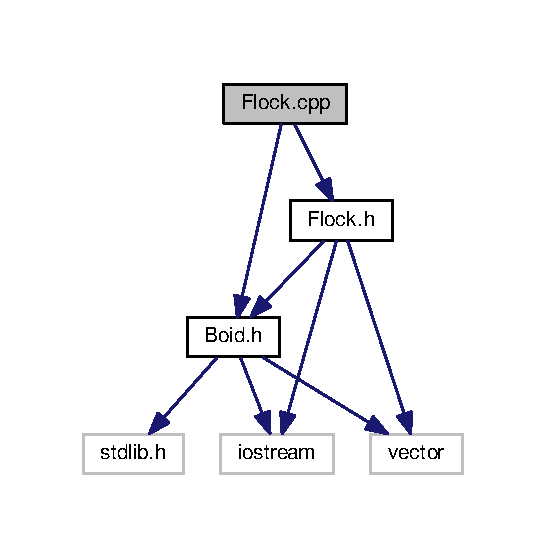
\includegraphics[width=262pt]{Flock_8cpp__incl}
\end{center}
\end{figure}

\hypertarget{Flock_8h}{}\section{Flock.\+h File Reference}
\label{Flock_8h}\index{Flock.\+h@{Flock.\+h}}
{\ttfamily \#include $<$iostream$>$}\\*
{\ttfamily \#include $<$vector$>$}\\*
{\ttfamily \#include \char`\"{}Boid.\+h\char`\"{}}\\*
Include dependency graph for Flock.\+h\+:\nopagebreak
\begin{figure}[H]
\begin{center}
\leavevmode
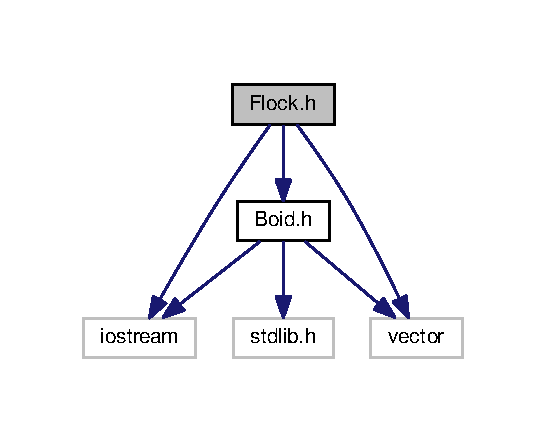
\includegraphics[width=262pt]{Flock_8h__incl}
\end{center}
\end{figure}
This graph shows which files directly or indirectly include this file\+:\nopagebreak
\begin{figure}[H]
\begin{center}
\leavevmode
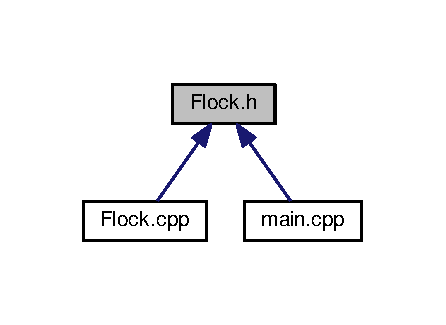
\includegraphics[width=214pt]{Flock_8h__dep__incl}
\end{center}
\end{figure}
\subsection*{Classes}
\begin{DoxyCompactItemize}
\item 
class \hyperlink{classFlock}{Flock}
\end{DoxyCompactItemize}

\hypertarget{main_8cpp}{}\section{main.\+cpp File Reference}
\label{main_8cpp}\index{main.\+cpp@{main.\+cpp}}
{\ttfamily \#include $<$iostream$>$}\\*
{\ttfamily \#include \char`\"{}Flock.\+h\char`\"{}}\\*
{\ttfamily \#include \char`\"{}Boid.\+h\char`\"{}}\\*
{\ttfamily \#include \char`\"{}S\+F\+M\+L/\+Window.\+hpp\char`\"{}}\\*
{\ttfamily \#include \char`\"{}S\+F\+M\+L/\+Graphics.\+hpp\char`\"{}}\\*
Include dependency graph for main.\+cpp\+:\nopagebreak
\begin{figure}[H]
\begin{center}
\leavevmode
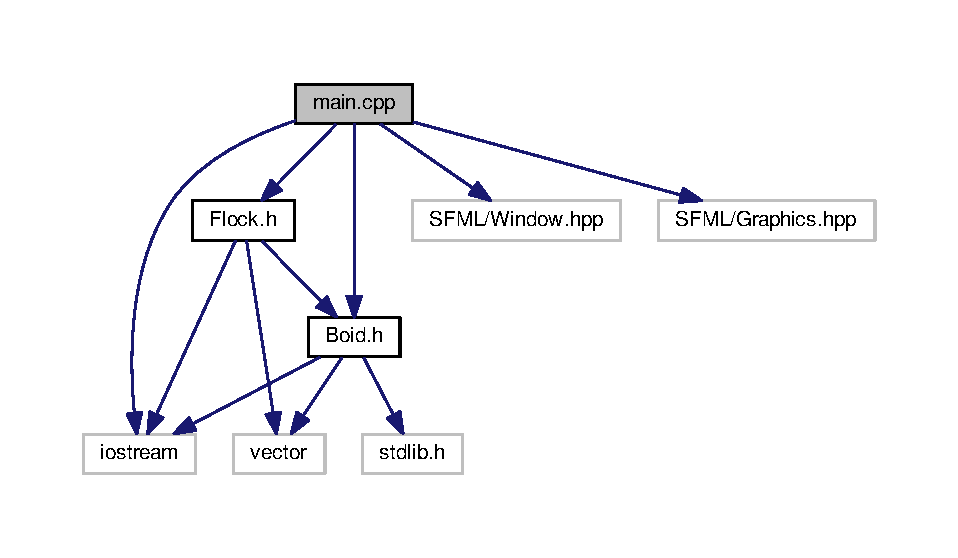
\includegraphics[width=350pt]{main_8cpp__incl}
\end{center}
\end{figure}
\subsection*{Classes}
\begin{DoxyCompactItemize}
\item 
class \hyperlink{classSimulate}{Simulate}
\end{DoxyCompactItemize}
\subsection*{Functions}
\begin{DoxyCompactItemize}
\item 
int \hyperlink{main_8cpp_ae66f6b31b5ad750f1fe042a706a4e3d4}{main} ()
\end{DoxyCompactItemize}


\subsection{Function Documentation}
\index{main.\+cpp@{main.\+cpp}!main@{main}}
\index{main@{main}!main.\+cpp@{main.\+cpp}}
\subsubsection[{\texorpdfstring{main()}{main()}}]{\setlength{\rightskip}{0pt plus 5cm}int main (
\begin{DoxyParamCaption}
{}
\end{DoxyParamCaption}
)}\hypertarget{main_8cpp_ae66f6b31b5ad750f1fe042a706a4e3d4}{}\label{main_8cpp_ae66f6b31b5ad750f1fe042a706a4e3d4}
The main function. Takes various inputs from the user for a better visualisation of simulation. Call the \hyperlink{classSimulate}{Simulate} class for execution which then takes care of subsequent simulation. \begin{DoxySeeAlso}{See also}
\hyperlink{classSimulate}{Simulate} 
\end{DoxySeeAlso}

%--- End generated contents ---

% Index
\backmatter
\newpage
\phantomsection
\clearemptydoublepage
\addcontentsline{toc}{chapter}{Index}
\printindex

\end{document}
